%!TEX TS-program = make
\documentclass[10pt, a4paper, twoside, english]{report}

%!TEX root = ../samlet.tex
\usepackage[applemac]{inputenc}
\usepackage[T1]{fontenc}
\usepackage{babel} %dansk sprog

%\DeclareGraphicsExtension{{pstex}}

\usepackage{ 
mathrsfs,
amsmath,
amssymb,
amsthm, % Definitions, theorms, lemmas
wasysym,
fancyhdr, %ja til fancy layout
fancyvrb, % bruges til noget kildekode haloej
listings, %kildekode viser
a4wide, %bred side
verbatim, %kode eksempel
subfigure,
rotating,
geometry,
minitoc,
stmaryrd,
pifont,
xspace,
upgreek,
booktabs,
multicol,
multirow,
mdwlist,
boxedminipage,
color,
float
}

\usepackage{harvard}

\usepackage{graphicx}
\graphicspath{{figurer/}}



%!TEX root = ./samlet.tex

\newcommand{\uppaal}{{\sc Uppaal}\xspace}
\newcommand{\forprojekt}{DHI og Aquaporin}



\textwidth 5.0in 
\oddsidemargin 1.0in
\evensidemargin 0.0in
\headwidth 5.0in
\def\test#1{\def\test{#1}}

% ------------------- configure mini toc ------------------------------
\setcounter{tocdepth}{1}        % setting depth of TOC
\dominitoc                      % enable minitoc
\setcounter{minitocdepth}{2}    % setting depth of miniTOC

% ------------------- configure biblograhystyle
%\bibliographystyle{alpha}
%\bibliographystyle{plain}
\bibliographystyle{agsm}

\harvardparenthesis{square}


% ------------------- hypernation rules --------------------------------
\hyphenation{Itera-tion}


% ------------------- configure logo image -------------------------------
\newsavebox{\auclogo}
\sbox{\auclogo}{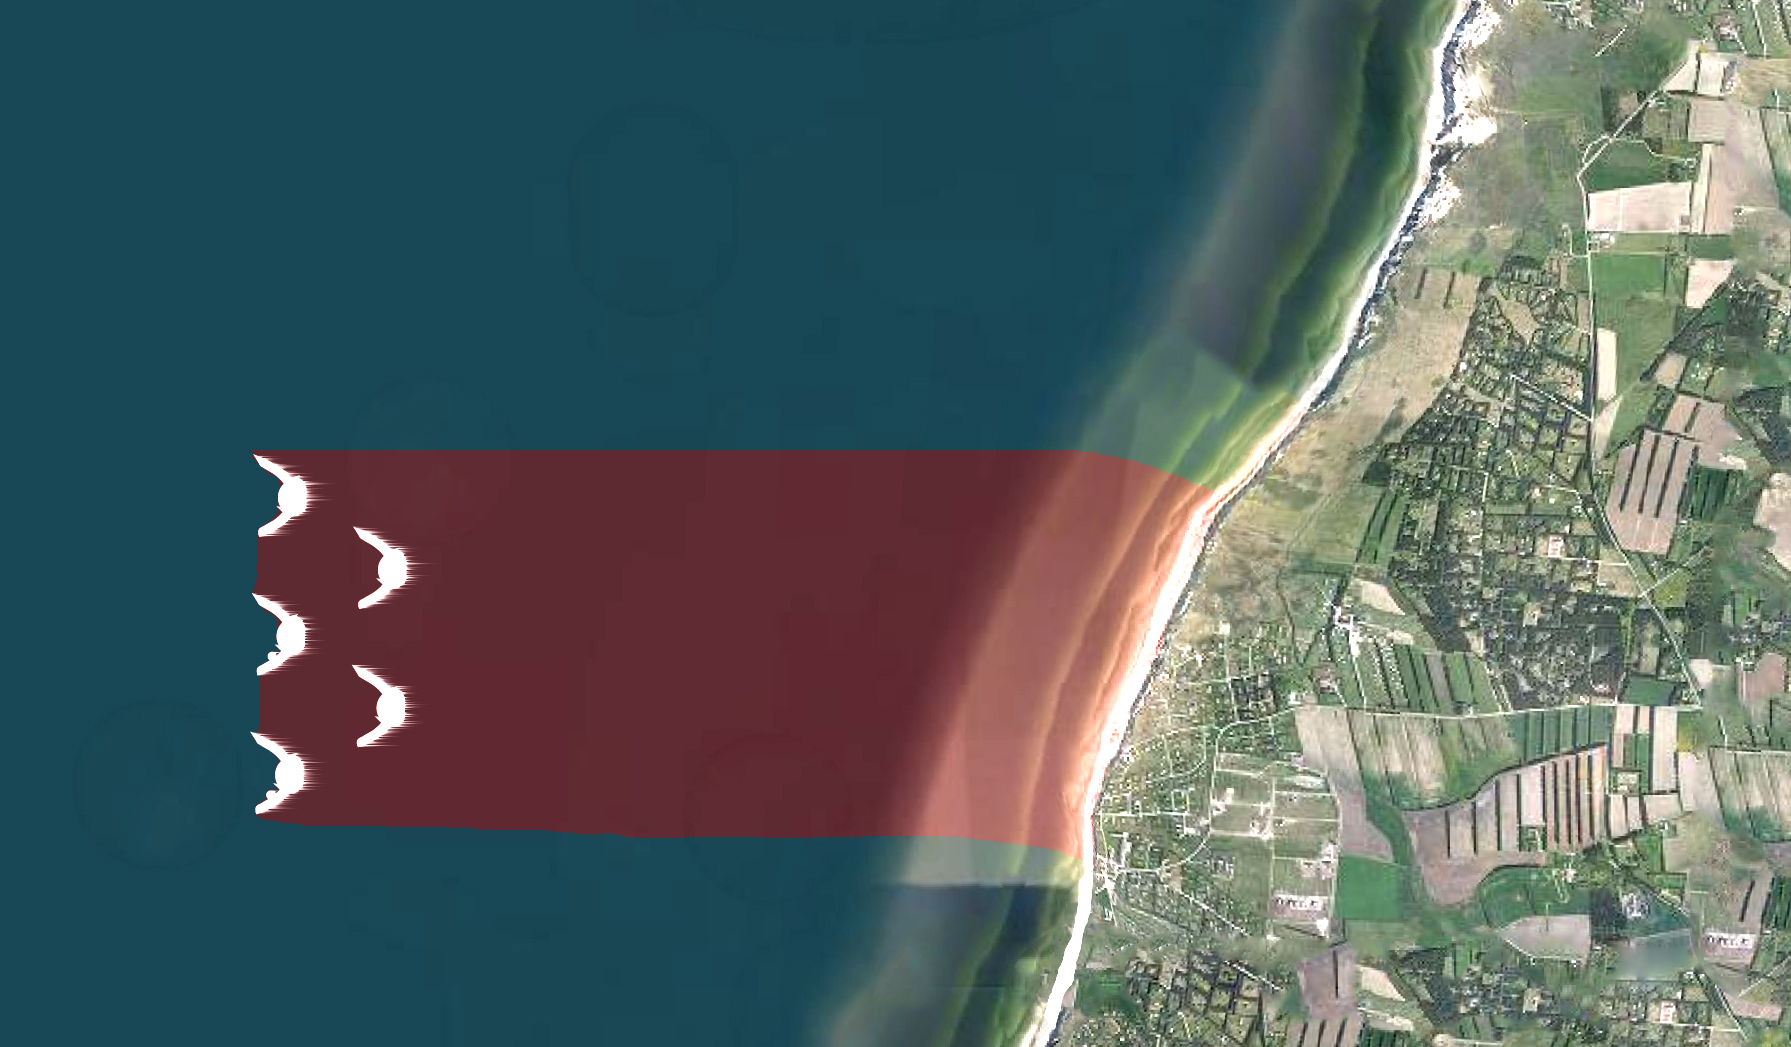
\includegraphics[totalheight=4mm]{figurer/forside_p3}}

%-------------------configurer fancy layout ------------------------------
\pagestyle{fancy} %aktiver fancy layout
\renewcommand{\chaptermark}[1]{\markboth{#1}{}} %g�r alle chapter overskrifter lowercase i headder
\renewcommand{\sectionmark}[1]{\markright{\thesection\ #1}} % g�r alle section overskriver lowercase

\fancyhf{} %reset settings til header og footer
%\fancyhead[C]{\usebox{\auclogo}} %placere auclogo i center af headder
\fancyhead[LE,RO]{\bfseries\thepage} %placere sidetal LE(left,even pages) RO(right,odd pages)
\fancyhead[LO]{\bfseries\rightmark} % placere section overskrift LO i headder
\fancyhead[RE]{\bfseries\leftmark} % placere chapter overskrift RE i headder

\renewcommand{\headrulewidth}{0.5pt}
\renewcommand{\footrulewidth}{0pt}
%\addtolength{\headheight}{0.5pt} %g�r plads til regel
\addtolength{\headheight}{24.26695pt}
\fancypagestyle{plain}{%
  \fancyhead{} %fjern headers p� normale sider
  \renewcommand{\headrulewidth}{0pt} %og p� linien
}
%---------------------fancy layout config stop ------------------------------


%---------------------smart forside
\makeatletter
\renewcommand{\maketitle}{\begin{titlepage}
   \hbox{
      \vrule depth 0.95\textheight 

      \vtop{
        \vskip 100\p@
        \begin{center} 
          \LARGE \bf \@title \par
          \vskip 20\p@
          \small \@author \par 
          \vskip 40\p@ \par
          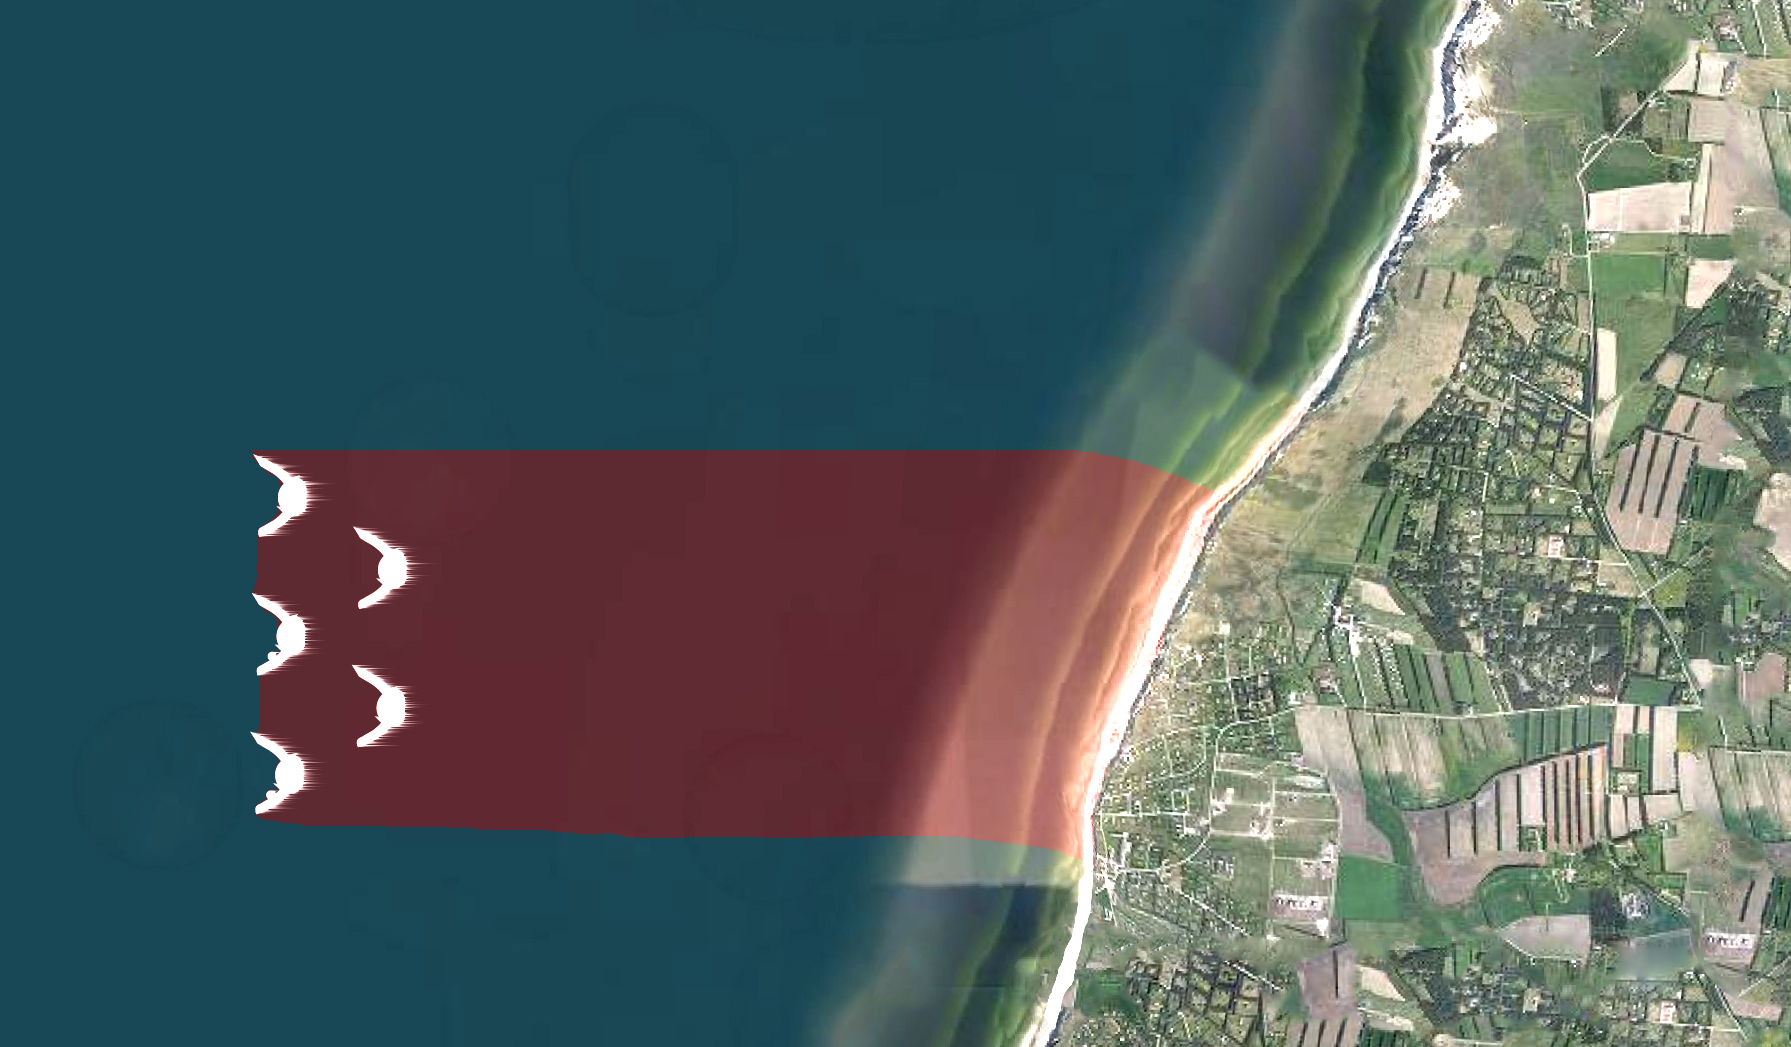
\includegraphics[scale=0.25]{figurer/forside_p3} \par  
	  \vskip 40\p@ \par        
          %\includegraphics[scale=0.6]{figurer/aau_logo} \par
          \small \@date
        \end{center}
       \vfil}
   }
   \pagestyle{empty}
   \cleardoublepage %making sure that the next page is clean
\end{titlepage}\setcounter{footnote}{0}}
%----------------------slut smart forside

%---------------------- smart chapter
\makeatletter
\def\@makechapterhead#1#2{\reset@font\parindent \z@\vspace*{10\p@}%
  \hbox{%

    \vbox{\hsize=2cm      
      \begin{tabular}{c}
        \scshape \strut \@chapapp{} \\
        \fbox{%
          \vrule depth 8em width 0pt%
          \vrule height 0pt depth 0pt width 1ex%
          {\LARGE \bfseries \strut \thechapter}%
          \vrule height 0pt depth 0pt width 1ex%
          }
      \end{tabular}}% vbox end

    \vbox{%
      \advance\hsize by -2cm
      \hrule\par
      \vskip 1pt%
      \hspace{1em}%
      \huge \bfseries #1
      \large \bfseries #2
      }% vbox end
    }% hbox end
  \vskip 10\p@
}
%---------------------- slut smart chapter


\DeclareFontFamily{OT1}{pzc}{}
\DeclareFontShape{OT1}{pzc}{m}{it}{<-> s * [0.900] pzcmi7t}{}
\DeclareMathAlphabet{\mathpzc}{OT1}{pzc}{m}{it}


\author{Bo S�rensen, Mikkel Laursen, Rick, test}

\date{3. Juni 2011}

\title{Diskursanalyse af Christania}

\begin{document}

\maketitle

%!TEX root = ../samlet.tex

\thispagestyle{empty}

{\samepage
%\setlength{\hoffset}{-2in}

\begin{tabular}{lc}
\parbox{5cm}{
%\hspace{2cm}

\begin{description}
\item {\Large Titel:} \newline \@title 
\item {\Large Tema:} \newline
Kulturgeografi:Diskursanalyse og byudvikling.
\end{description}

\parbox{5cm}{
\begin{description}
\item {\Large Projektramme:}\smallskip \newline
  P4\newline
  2. Feb - 3. Juni, 2011\smallskip \newline
  \hspace{4cm}
\item {\Large Forfattere:}\smallskip \newline
Bo S�rensen\newline
Kristian Wost Snapsensen\newline
Ronni Fjordvald S�e 
  \newline
  \hspace{2cm}
\item {\Large Vejleder:}\smallskip \newline
 Anne Lorensen. \newline
% \item {\Large Bivejleder:}\smallskip \newline
  \newline
\end{description}
}
\begin{description}
\item {\bf Oplagstal:}  
\item {\bf Sidetal:}  
\item {\bf Bilagsantal og --art:}  
\item {\bf Afsluttet den} 3. Juni. 2011.
\end{description}

\vfill } &

\parbox{5cm}{
  \vspace{.15cm}
  \flushright
  \fbox{
    \parbox{8cm}{{\bf Synopsis} \vspace{0.5cm}
    \vfill
    \small
    %!TEX root = ../samlet.tex

Snaps 
 



    }\vspace{0.5cm}
     }
}
\end{tabular}
}
\\ \\
\noindent{\footnotesize\emph{Rapportens indhold er frit tilg�ngeligt, men offentligg�relse (med kildeangivelse) m� kun ske efter aftale med forfatterne.}}
\vspace{1.2cm}
\newpage
\thispagestyle{empty}
\newpage

\cleardoublepage

%!TEX root = ../samlet.tex

\begin{description}
\item \Large{Forord}\newline
\end{description}
\cleardoublepage

\cleardoublepage
\tableofcontents
\thispagestyle{empty}
\cleardoublepage

\chapter{Introduktion}{%!TEX root = ../samlet.tex

Dette kapitel giver en kort introduktion til projektet, og pr�senterer selve problemformuleringen samt afgr�nsningen. Sidst i kapitlet findes en beskrivelse af den anvendte metode og en oversigt over opbygningen af projektet.

\minitoc
\newpage
}\label{chap:introduktion}\newpage
%!TEX root = ../samlet.tex

%!TEX root = ../samlet.tex

\section{Indledning}
Do the wost thing... Yes





%!TEX root = ../samlet.tex

\section{Problemformulering}






%!TEX root = ../samlet.tex

\section{Afgr�nsning}






















%!TEX root = ../samlet.tex

\section{Metode}

det er bare for grove
%!TEX root = ../samlet.tex

\section{Opbygning}

 







\clearpage
\newpage
\thispagestyle{empty}
\cleardoublepage
\newpage


\chapter{Teori}{%!TEX root = ../samlet.tex



\minitoc
\newpage


}\label{chap:teori}\newpage
%!TEX root = ../samlet.tex



\clearpage
\newpage
\thispagestyle{empty}
\cleardoublepage
\newpage


\chapter{Diskursanalyse}{%!TEX root = ../samlet.tex



 

\minitoc
\newpage

}\label{chap:diskursanalyse}\newpage
%!TEX root = ../samlet.tex

%!TEX root = ../samlet.tex

\section{Jep}






















 
























\clearpage
\newpage
\thispagestyle{empty}
\cleardoublepage
\newpage



\chapter{Konlusion}{%!TEX root = ../samlet.tex




\minitoc
\newpage
}\label{chap:konklusion}\newpage
%!TEX root = ../samlet.tex



%!TEX root = ../samlet.tex

\section{Diskussion}


%!TEX root = ../samlet.tex

\section{Konklusion}




\clearpage
\newpage
\thispagestyle{empty}
\cleardoublepage
\newpage


%\appendix
%\chapter{Appendiks}{%!TEX root = ../samlet.tex


\minitoc
\newpage
}\label{chap: appendix}\newpage
%%!TEX root = ../samlet.tex

\input{appendix/istid}
\input{appendix/metrologi}



%\clearpage
%\newpage
%\thispagestyle{empty}
%\cleardoublepage
%\newpage






\small{
\renewcommand{\bibname}{Referencer}
\bibliography{bibliography}
}
\clearpage
\newpage
\thispagestyle{empty}
\cleardoublepage
\newpage

\end{document}
